% Absolute Encoder
% Author: Germain Gondor
% https://gondor-carnot.fr
\documentclass[border=10pt]{standalone}
\usepackage{tikz}
\begin{document}
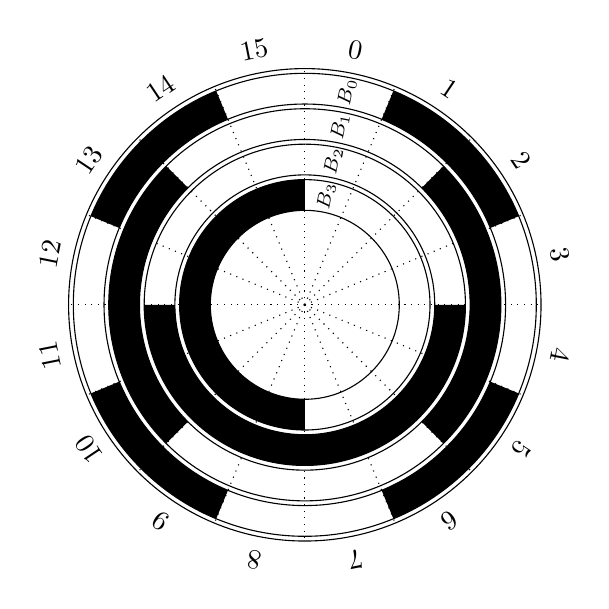
\begin{tikzpicture}
  \def\R{3} % Radius
  \def\basea{22.5} % 360/(2^4)

  % Big circle and numbering
  \draw circle(\R); 
  \foreach \x in {0,\basea, ..., 359}
    {\draw [dotted](0,0)--(\x:\R);} % draw radius
  \foreach \x in {0,...,15}
    {\pgfmathsetmacro\ang{-(\x+0.5)*\basea} % calculate position
    \node at({90-(\x+0.5)*\basea}:1.1*\R)[rotate=\ang]{\x};} % numbering

  % Circles 
  \foreach \x in {40,53, 55,68,70,83,85,98} % Diameters
  {\draw circle({\x*\R/100});}

  % B3
  \fill (4*\basea:0.53*\R)arc(4*\basea:12*\basea:0.53*\R)
	--(12*\basea:0.40*\R)arc(12*\basea:4*\basea:0.40*\R)--cycle;

  % B2
  \fill (8*\basea:0.68*\R)arc(8*\basea:16*\basea:0.68*\R)
	--(16*\basea:0.55*\R)arc(16*\basea:8*\basea:0.55*\R)--cycle;

  % B1
  \foreach \x in {0,1}
  {\fill ({4*(1.5+\x*2)*\basea}:0.83*\R)
	arc({4*(1.5+\x*2)*\basea}:{4*(2.5+\x*2)*\basea}:0.83*\R)
	--({4*(2.5+\x*2)*\basea}:0.70*\R)
	arc({4*(2.5+\x*2)*\basea}:{4*(1.5+\x*2)*\basea}:0.70*\R)--cycle;}

  % B0
  \foreach \x in {0,...,3}
  {\fill ({2*(0.5+\x*2)*\basea}:0.98*\R)
	arc({2*(0.5+\x*2)*\basea}:{2*(1.5+\x*2)*\basea}:0.98*\R)
	--({2*(1.5+\x*2)*\basea}:0.85*\R)
	arc({2*(1.5+\x*2)*\basea}:{2*(0.5+\x*2)*\basea}:0.85*\R)--cycle;}

  % legends
  \pgfmathsetmacro\ang{90-0.5*\basea} % to rotate B_i
  \begin{scope}[font=\scriptsize]
    \node at ({90-\basea/2}:0.47*\R)[rotate=\ang]{$B_3$};
    \node at ({90-\basea/2}:0.62*\R)[rotate=\ang]{$B_2$};
    \node at ({90-\basea/2}:0.77*\R)[rotate=\ang]{$B_1$};
    \node at ({90-\basea/2}:0.92*\R)[rotate=\ang]{$B_0$};
  \end{scope}
\end{tikzpicture}
\end{document}